\chapter{Additional Experimental Results}
\label{app:results}

\TODO{marker=DAG\_EXAMPLE to refer back to this figure from the main text (Section~\ref{sec:model:dag})}
\begin{figure}[ht]
    \centering
    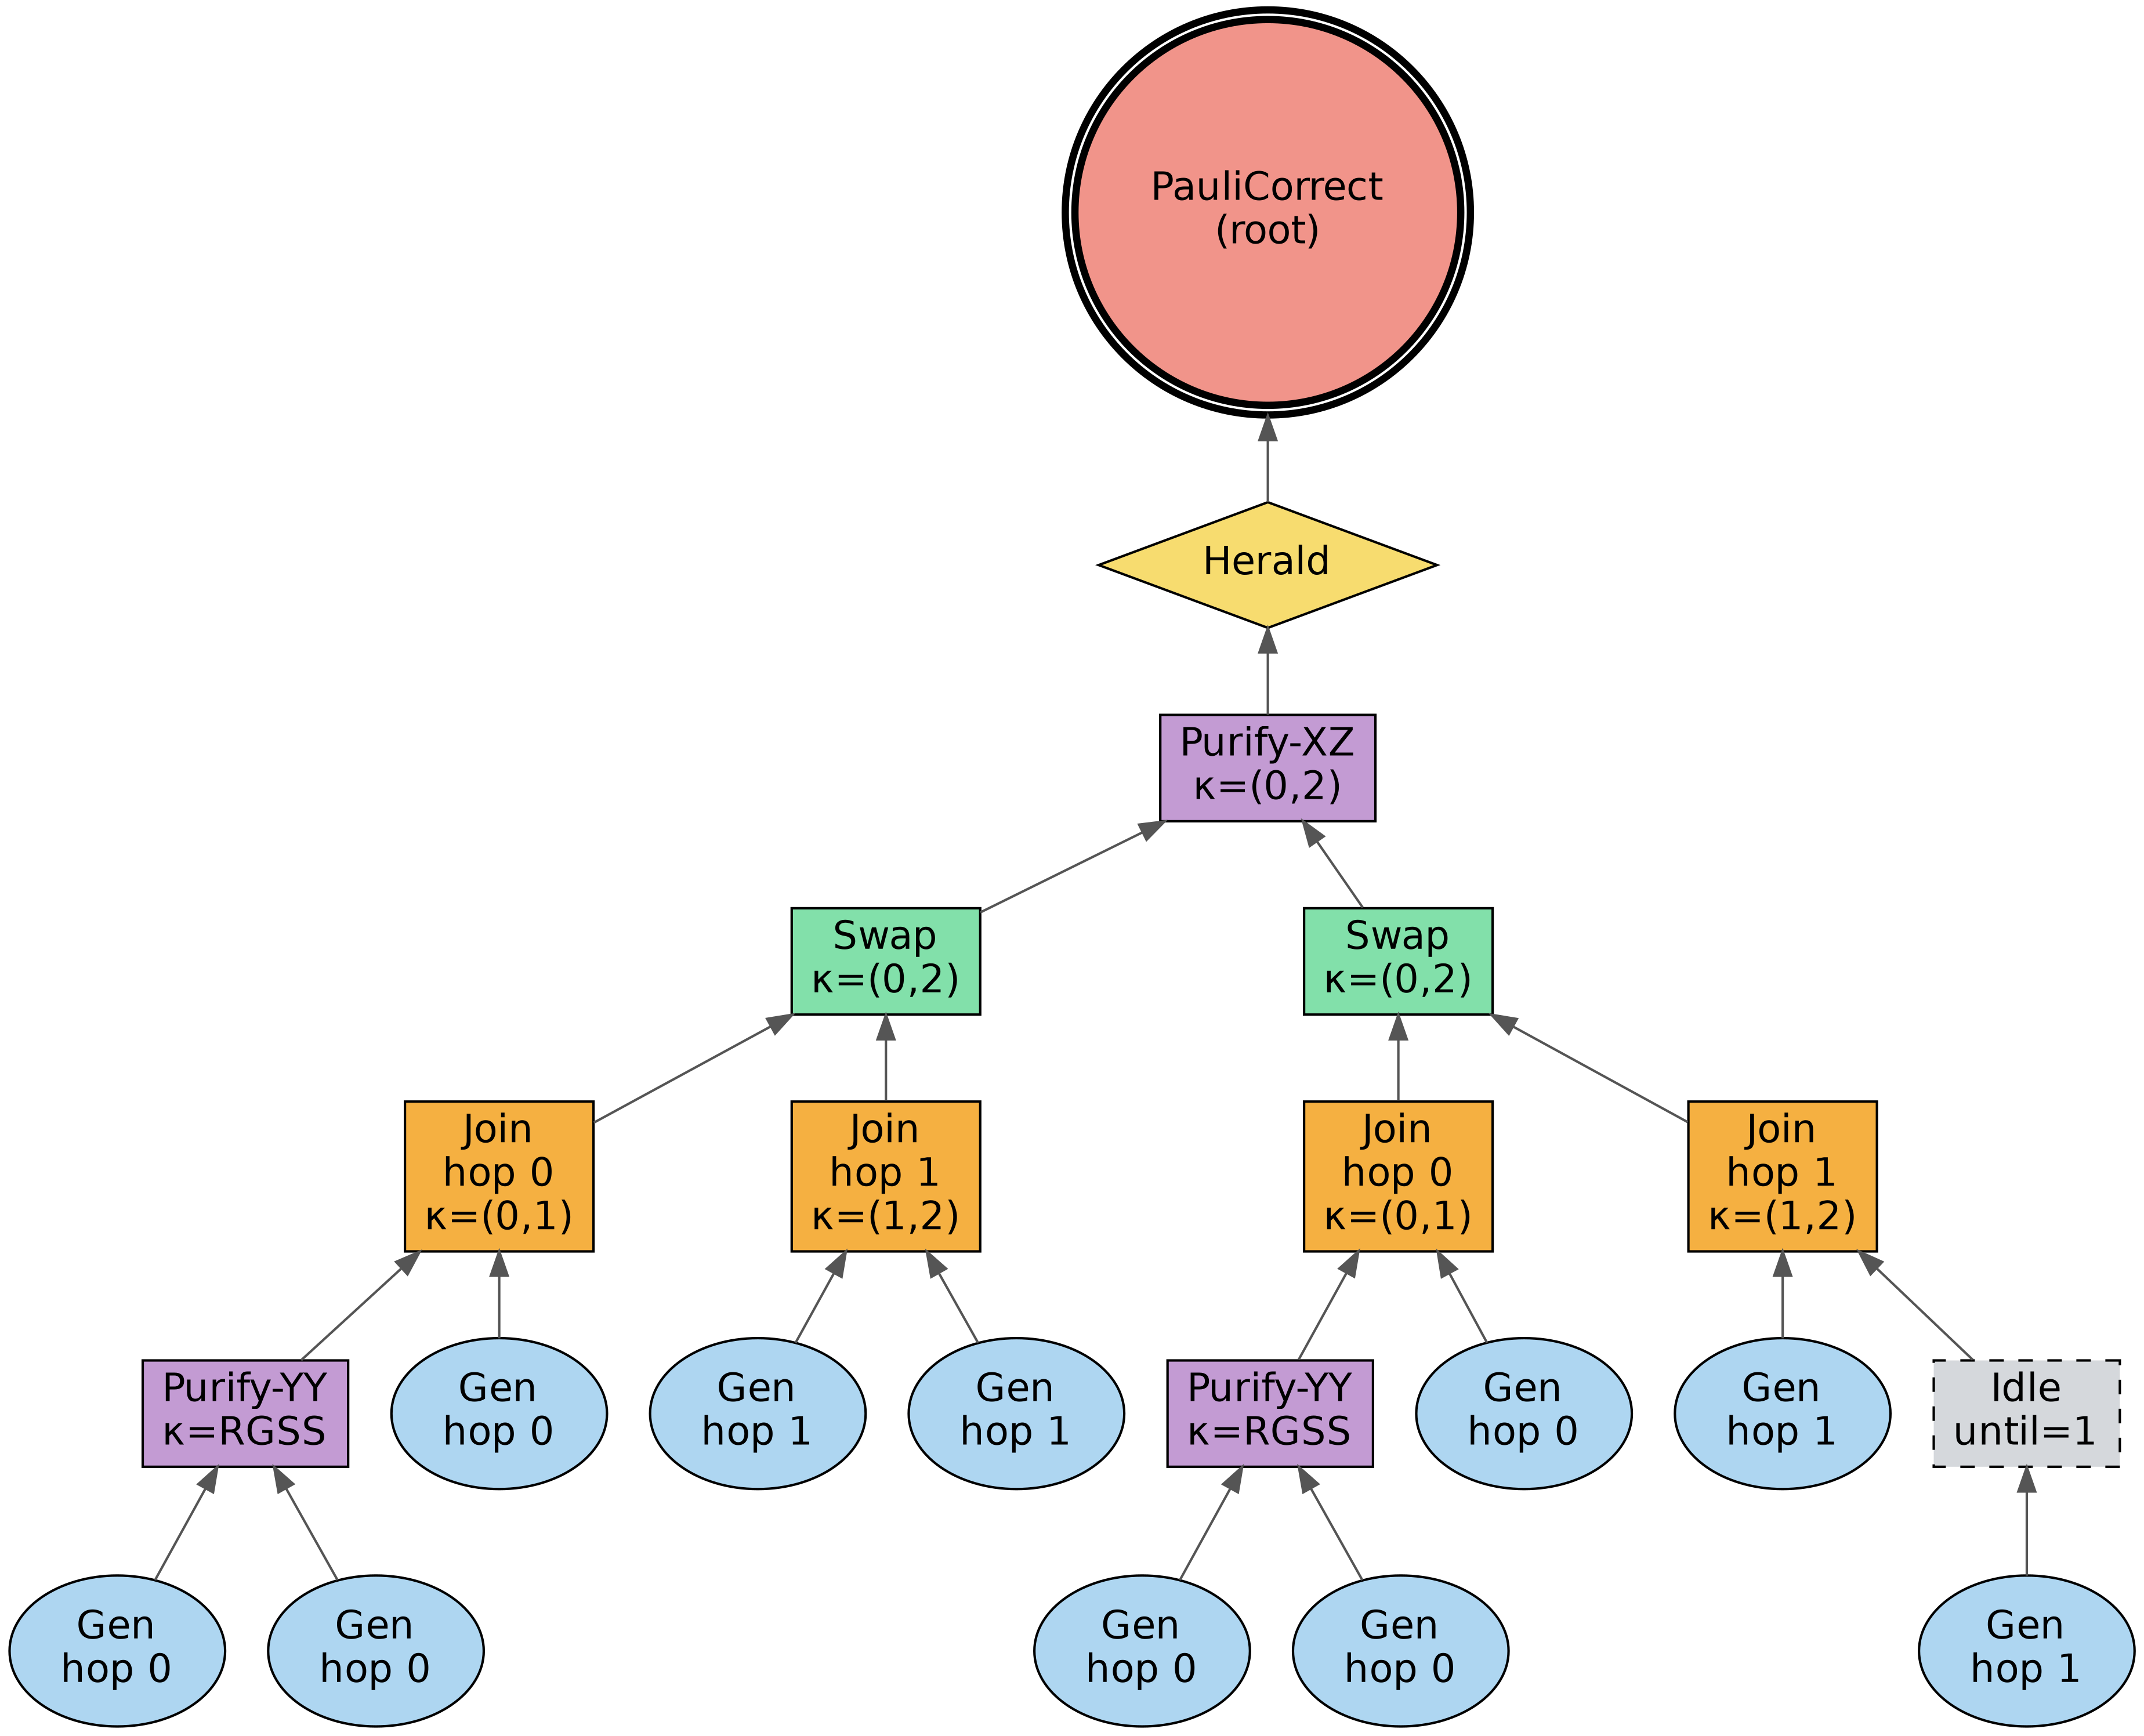
\includegraphics[width=0.95\textwidth]{figures/method/dag_n2_worked_example.png}
    \caption{\small%
        $N=2$ example schedule $\Sigma$ illustrating all seven node types ($C(\Sigma)=10$ \texttt{GenNode} leaves).
        \textbf{Copy~A} (left subtree): hop~0 applies \texttt{PurifyNode-YY} at $\kappa=\mathrm{RGSS}$ before the outer-photon \texttt{JoinNode}; hop~1 is raw.
        \textbf{Copy~B} (right subtree): identical except the right-side hop-1 \texttt{GenNode} is wrapped in an \texttt{IdleNode} (grey, dashed) modelling a synchronisation wait before the \texttt{JoinNode}.
        The two copies are first combined into $\kappa=(0,2)$ by a \texttt{SwapNode}, then purified together by \texttt{PurifyNode-XZ}.
        The single \texttt{HeraldNode} placed after (not before) \texttt{PurifyNode-XZ} makes this an optimistic schedule (Section~\ref{sec:model:dag}).
        \texttt{PauliCorrectNode} is the root at $\kappa=(0,2)$. Edges run bottom-to-top.
    }
    \label{fig:model:dag-example}
\end{figure}

\section{Validation Figures}
\label{app:validation}

Section~\ref{sec:exp:validation} reports the evaluator's agreement with the source paper's Fig.\,5 at its single published headline point, $e_d=0.01$. Table~\ref{tab:app:validation} gives the evaluator's fidelity output for the raw, heralded-pumping, and optimistic-pumping canonical schedules (Section~\ref{sec:bg:decoherence}) across the full $e_d \in [0, 0.01]$ grid used throughout Chapter~\ref{chap:results}, rather than only at that one point.

The source paper publishes numeric reference values at only two points on this grid, $e_d=0.000$ and $e_d=0.010$: approximately $\{1.000, 1.000, 1.000\}$ and $\{0.823, 0.917, 0.929\}$ respectively, for the same three schedules in the same order. The evaluator matches both to at least three significant figures, and to four at $e_d=0.010$ (the values already quoted in Section~\ref{sec:exp:validation}). The nine intermediate rows have no corresponding published value to compare against, since the source paper's own Fig.\,5 does not report numeric values between its two published points; they are included here as the exact evaluator output behind every noise-swept result in this thesis, not as a further reproduction check.

\begin{table}[h]
\centering
\caption{Evaluator-derived fidelity vs.\ $e_d$ for the three canonical schedules of Section~\ref{sec:bg:decoherence}, at $N=10$. Only $e_d=0.000$ and $e_d=0.010$ have a published reference value to compare against (see text).}
\label{tab:app:validation}
\small
\begin{tabular}{cccc}
\hline
$e_d$ & $F_{\text{raw}}$ & $F_{\text{baseline (heralded)}}$ & $F_{\text{flexible (optimistic)}}$ \\
\hline
0.000 & 1.0000 & 1.0000 & 1.0000 \\
0.001 & 0.9803 & 0.9932 & 0.9933 \\
0.002 & 0.9610 & 0.9861 & 0.9866 \\
0.003 & 0.9422 & 0.9787 & 0.9799 \\
0.004 & 0.9239 & 0.9710 & 0.9730 \\
0.005 & 0.9061 & 0.9629 & 0.9661 \\
0.006 & 0.8887 & 0.9544 & 0.9591 \\
0.007 & 0.8717 & 0.9456 & 0.9519 \\
0.008 & 0.8552 & 0.9364 & 0.9446 \\
0.009 & 0.8391 & 0.9268 & 0.9372 \\
0.010 & 0.8234 & 0.9168 & 0.9295 \\
\hline
\end{tabular}
\end{table}

\section{Schedule DAGs of Selected Optima}
\label{app:dags}

The schedules found in Chapter~\ref{chap:results}, such as the budget-relaxed optimum at $N=10$ (Section~\ref{sec:exp:headline}), are automatically constructed \Glspl{dag} with 50 to 100 \texttt{GenNode} leaves and several hundred nodes once every backbone and purification step is counted. Rendered at a scale where individual node labels stay legible, such a diagram does not fit within a single printed page: the same rendering tooling used for the worked $N=2$ example of Figure~\ref{fig:model:dag-example} produces images several thousand pixels wide once applied to these larger, automatically-constructed schedules, since node count (not page size) is the limiting factor.

Reproducing one of these diagrams here at a reduced scale would not add information beyond what Chapter~\ref{chap:results}'s tables and the Pareto frontier of Figure~\ref{fig:pareto} already convey, namely each schedule's cost, fidelity, rate, and overall shape family (e.g.\ end-node pumping vs.\ a span-partition structure), while making every individual node illegible. Figure~\ref{fig:model:dag-example} therefore remains the representative illustration of the \Gls{dag} representation itself, at a size deliberately chosen to exercise every node type from Section~\ref{sec:model:dag} while staying legible; the full artifacts for every optimum discussed in this thesis are reproducible directly from the search calls and parameters documented in Chapter~\ref{chap:algorithms} and Table~\ref{tab:params}.

\section{Supplementary Sweep Figures}
\label{app:sweeps}

These figures support the runtime and determinism claims of Section~\ref{sec:exp:runtime} and Table~\ref{tab:runtimes}, without interrupting the main narrative of Chapter~\ref{chap:results}.

Figure~\ref{fig:app:beamwidth} shows why beam width $w_\text{beam}=25$ was chosen as the default used throughout this thesis: at $N=10$, wall-clock search time grows mildly up to a beam width of about 16 and then sharply beyond it, while the best rate found is already flat across the entire tested range, so widening the beam past 25 buys no further quality improvement at this configuration.

\begin{figure}[ht]
    \centering
    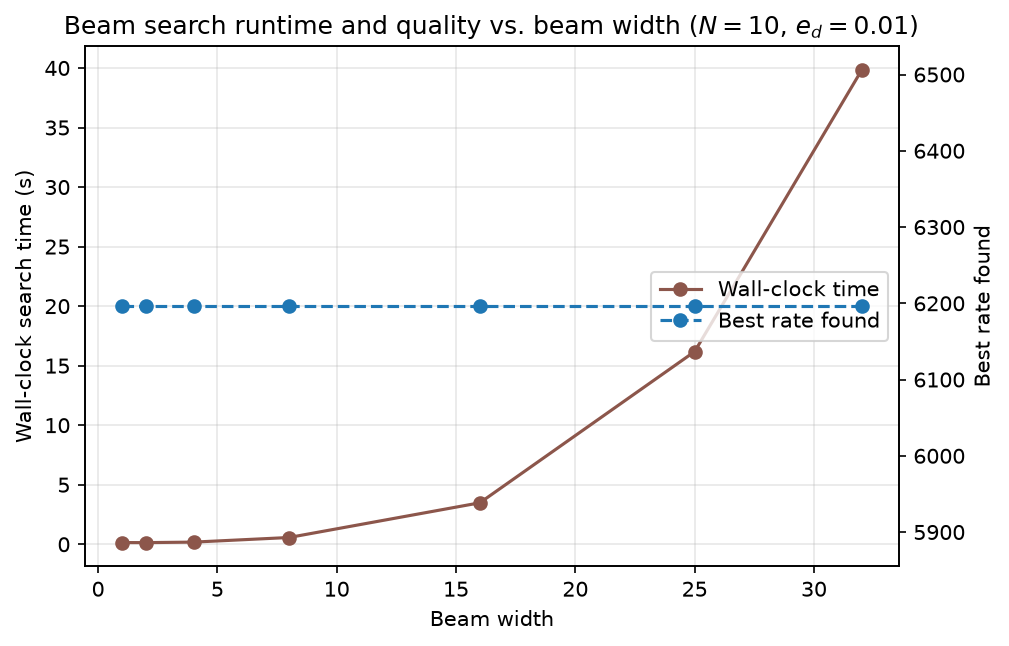
\includegraphics[width=0.75\textwidth]{figures/appendix/runtime_and_quality_vs_beam_width.png}
    \caption{Beam search wall-clock time and best rate found vs.\ beam width, at $N=10$, $e_d=0.01$.}
    \label{fig:app:beamwidth}
\end{figure}

Figure~\ref{fig:app:qualitygap} confirms the determinism claim underlying that choice: at $N=6$, where the exact dynamic program (Section~\ref{sec:alg:dp}) remains tractable, the beam search matches the exact optimum exactly at every beam width tested, with a zero gap throughout.

\begin{figure}[ht]
    \centering
    
\includegraphics[width=0.75\textwidth]{figures/appendix/quality_gap_vs_beam_width.png}
    \caption{Beam search's rate gap from the exact dynamic-program optimum vs.\ beam width, at $N=6$, $e_d=0.01$.}
    \label{fig:app:qualitygap}
\end{figure}

Figure~\ref{fig:app:runtimen} extends the runtime comparison of Table~\ref{tab:runtimes} to every tested $N$: both the exact dynamic program and the beam search scale similarly with $N$ once the same-span pumping move (Section~\ref{sec:alg:pumping}) is enabled, with the beam search consistently the faster of the two.

\begin{figure}[H]
    \centering
    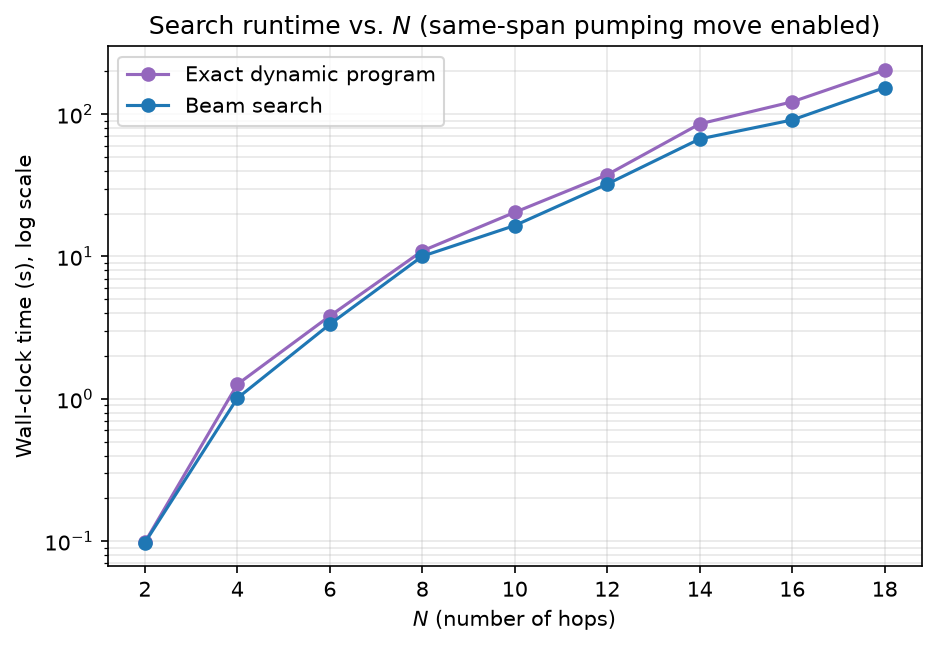
\includegraphics[width=0.75\textwidth]{figures/appendix/runtime_vs_n_pumping.png}
    \caption{Search wall-clock time vs.\ $N$ for the exact dynamic program and the beam search, same-span pumping move enabled throughout.}
    \label{fig:app:runtimen}
\end{figure}

\subsection{Concurrent Branch Budget ($M_{\max}$)}
\label{app:mmax}

Section~\ref{sec:model:scope} notes that $M_{\max}$, the number of concurrently open branches (Section~\ref{sec:model:budget}), is computed exactly for a given schedule but is not used to prune the search itself. Table~\ref{tab:app:mmax} gives $M(\Sigma)$ for the fixed schedule families and the optimizer's own budget-relaxed best schedule across $N=2$ to $N=18$ at $e_d=0.01$: no family shows $M(\Sigma)$ growing with $N$, since the register-allocation bound (Section~\ref{sec:model:budget}) is governed by \Gls{dag} depth and branching shape rather than hop count. Bisecting $m_{\max}$ downward from the unconstrained optimum at $N=10$, $E_{\max}=100$ shows that the budget-relaxed optimum ($M=4$) remains selectable down to $m_{\max}=4$, but no candidate in the beam-searched frontier clears both the rate objective and $m_{\max}=3$, at which point $M_{\max}$ becomes the actual binding constraint rather than $E_{\max}$ or $F_{\min}$.

\begin{table}[h]
    \centering
    \caption{$M(\Sigma)$ vs.\ $N$ for the fixed schedule families and the budget-relaxed optimum, $e_d=0.01$.}
    \label{tab:app:mmax}
    \small
    \begin{tabular}{cccc}
        \hline
        $N$ & Raw chain & Heralded end-node pumping & Optimizer (budget-relaxed) \\
        \hline
        2  & 3 & 4 & 3 \\
        4  & 3 & 4 & 4 \\
        6  & 3 & 4 & 4 \\
        8  & 3 & 4 & 4 \\
        10 & 3 & 4 & 4 \\
        14 & 3 & 4 & 4 \\
        18 & 3 & 4 & 5 \\
        \hline
    \end{tabular}
\end{table}

\section{Alternative Objectives, Full Comparison}
\label{app:objectives}

Section~\ref{sec:exp:objectives} summarizes the objective-substitution result; Table~\ref{tab:app:objectives} gives the full five-objective comparison it draws from, at $N=10$ and $e_d=0.01$.

\begin{table}[h]
    \centering
    \caption{Objective-substitution comparison at $N=10$, $e_d=0.01$: five objective definitions with no change to the search algorithm.}
    \label{tab:app:objectives}
    \small
    \begin{tabular}{lccc}
        \hline
        Objective & $C$ & $F$ & Rate \\
        \hline
        Maximize rate & 60 & 0.9063 & 6195.95 \\
        Maximize fidelity, paper-rate floor & 80 & 0.9351 & 4804.58 \\
        Maximize fidelity, matched-rate floor & 80 & 0.9351 & 4804.58 \\
        Minimize cost, $F \ge 0.9$ only & 60 & --- & 1239.19 \\
        Minimize cost, $F \ge 0.9$ and $R \ge 4055.92$ & 60 & --- & 6195.95 \\
        \hline
    \end{tabular}
\end{table}

\section{Optimality Bound at $N=18$}
\label{sec:exp:excluded}

% Source: outputs/excluded_move_n14_n18/README.md,
%          docs/Optimality Scope.md

Section~\ref{sec:exp:budget} bisects the minimum feasible budget within the schedule families the search actually considers. This section checks that bound against one schedule outside those families, at the single point where Section~\ref{sec:exp:budget}'s crossover analysis is most sensitive to it, $N=18$.

A hand-constructed schedule using a same-span construction excluded from the search (purifying two independently constructed $\mathrm{Span}(0,18)$ resources) achieves $F=0.93$ at $E_{\max}=180$, the paper's own budget for $N=18$. The beam search cannot reach this schedule even with same-span pumping enabled (Section~\ref{sec:alg:pumping}), because that construction lies outside the schedule families it considers.

This is an optimality-scope result, not a scalability result: it demonstrates that the searched families do not cover the full legal schedule space, consistent with the scope stated in Section~\ref{sec:model:scope}, and gives a concrete example of why the bounded-search results of Section~\ref{sec:exp:budget} must not be read as proofs of global optimality.

\section{Timing Sensitivity, Full Sweeps}
\label{app:timing}

% Source: outputs/sweep_gamma_and_tau_emit/README.md

Section~\ref{sec:exp:timing} summarizes the effect of memory dephasing and generation latency on schedule rate and fidelity; Figure~\ref{fig:timing} gives both sweeps in full, at $N=10$ and $e_d=0.01$.

\paragraph{Memory dephasing ($\gamma$)}

Sweeping $\gamma$ from 0 to $10^5$ leaves the raw chain and paper schedule's fidelity unchanged across the tested range: neither contains a resource that waits for another branch to become ready, so the simulated execution introduces no additional memory-decoherence interval for these schedules. By contrast, heralded end-node pumping falls from $F=0.92$ at $\gamma=0$ to $F=0.25$, the maximally mixed limit, at $\gamma=10^5$, because its sacrificial copies remain stored while each round-trip heralding delay is incurred. The schedules selected by the optimizer remain flat across the tested values of $\gamma$; this does not mean memory dephasing is generally harmless, only that the search favours optimistic schedules in which the relevant intermediate heralding delays are deferred, avoiding the specific waiting pattern that causes the collapse of the heralded pumping schedule (Section~\ref{sec:disc:optimistic}).

\paragraph{Generation latency ($\tau_{\mathrm{emit}}$)}

Sweeping $\tau_{\mathrm{emit}}$ at $\gamma=0$ reduces the rate monotonically for every schedule. The relative rate loss is largest for the optimistic pumping family, whose baseline latency is approximately $1\times L/c$, and smallest for heralded end-node pumping, whose baseline latency is approximately $9\times L/c$: a schedule that already has a larger fixed latency is proportionally less affected by the same additional per-photon generation delay. The two schedules cross near $\tau_{\mathrm{emit}}\approx0.01$; above this value, the larger fixed latency of heralded pumping makes it less sensitive, in relative terms, to further increases in generation latency.

\begin{figure*}[ht]
    \centering
    \begin{subfigure}[b]{0.48\textwidth}
        \centering
        
\includegraphics[width=\textwidth]{figures/results/gamma_fidelity.png}
        \caption{Fidelity vs.\ $\gamma$}
    \end{subfigure}
    \hfill
    \begin{subfigure}[b]{0.48\textwidth}
        \centering
        
\includegraphics[width=\textwidth]{figures/results/tau_emit_rate.png}
        \caption{Rate vs.\ $\tau_{\mathrm{emit}}$ (log-log)}
    \end{subfigure}
    \caption{Timing sensitivity of the raw chain, the paper schedule, and heralded end-node pumping, at $N=10$ and $e_d=0.01$.}
    \label{fig:timing}
\end{figure*}




%%%% TO REMOVE & REORGANIZE PROPERLY ONCE CHAPTER 6 IS DONE
% table here so as not to fuck up the references

\TODO{moved table to appendix in dedicated section (PARAMETERS)}
\begin{table}[ht]
    \centering
    \small
    \begin{tabular}{p{5cm}lllp{3cm}}
        \toprule
        Parameter & Symbol & Reference ($\mathcal{N}_{\mathrm{ref}}$) & Swept ranges & Where varied \\
        \midrule
        Hop count & $N$ & 10 & 10--28 & Section~\ref{sec:exp:budget} \\
        Hop length & $\ell_i$ & 2~km & \{1, 2, 3, 4\}~km & Section~\ref{sec:exp:heterogeneous} \\
        Tree-encoding branching vector & $\vec b^{(i)}$ & $(16,14,1)$ & -- & not varied \\
        BSM arm count & $k_i$ & 18 & 6, 18 & Section~\ref{sec:exp:netgen} \\
        Inner-qubit error rates & $\{p_X^{\mathrm{in}},p_Z^{\mathrm{in}}\}_i$ & 0 & [0, $3\!\times\!10^{-3}$] & Section~\ref{sec:exp:netgen} \\
        Photon survival probability & $\eta_i$ & 0.912 & $10^{-0.2 \ell_i/10}$ & Section~\ref{sec:exp:heterogeneous} \\
        Outer-photon depolarizing rate & $e_d$ & 0.01 & $[0,\,0.01]$ & Section~\ref{sec:exp:edsweep} \\
        Memory dephasing rate & $\gamma$ & 0 & $[0,\,10^5]$ & Section~\ref{sec:exp:timing} \\
        Propagation speed & $c$ & $2\!\times\!10^5$~km/s & -- & not varied \\
        Emission delay & $\tau_{\mathrm{emit}}$ & 0 & $[10^{-4},\,1]$ & Section~\ref{sec:exp:timing} \\
        Generation-cost budget & $E_{\max}$ & 100 & 50--280 & Sections~\ref{sec:exp:headline}--\ref{sec:exp:budget} \\
        \bottomrule
    \end{tabular}

    \caption{Experimental parameters. The reference column gives the nominal value used unless a parameter is varied in the indicated experiment. All parameters not listed as varying follow the Integrating paper's~\cite{Benchasattabuse2025Integrating} reference configuration $\mathcal{N}_{\mathrm{ref}}$ (Section~\ref{sec:model:network}). The tree branching factor is not varied because it does not affect the objectives $F$, $C$, or $R$ introduced in Chapter~\ref{chap:model}. Uniform hop-length scaling likewise leaves relative schedule comparisons unchanged; heterogeneous hop lengths are considered separately in Section~\ref{sec:exp:heterogeneous}.}
    \label{tab:params}
\end{table}

\TODO{moved table to appendix in dedicated section (BENCHMARKS)}
\begin{table}[ht]
    \centering
    \small
    \begin{tabular}{rrllrr}
        \toprule
        $N$ & $E_{\max}$ & Exact DP (s) & Beam search (s) & Exact DP score & Beam search score \\
        \midrule
        2  & 20  & 0.10 & 0.10 & 50\,000 & 50\,000 \\
        6  & 60  & 3.82 & 3.34 & 14\,372\textsuperscript{$\ddagger$} & 15\,391 \\
        10 & 100 & 20.43 & 16.50 & 6\,196 & 6\,196 \\
        14 & 140 & 85.37 & 66.93 & 3\,394 & 3\,394 \\
        18 & 180 & 203.68\textsuperscript{$\dagger$} & 153.52 & $-\infty$ & 1\,214 \\
        \bottomrule
    \end{tabular}

    \caption{Wall-clock runtime and returned score for the exact dynamic program and beam search at representative chain lengths. Runs use $E_{\max}=10N$, $F_{\min}=0.9$, beam width $w_{\mathrm{beam}}=25$, same-span pumping enabled (Section~\ref{sec:alg:pumping}), a 300~s timeout, and a 3~GiB memory limit. The score is the value of the active objective; here, it is the returned schedule rate $R(\Sigma)$. \textsuperscript{$\dagger$}At $N=18$, the exact dynamic program completes within the timeout but finds no feasible candidate, while beam search returns a feasible one. \textsuperscript{$\ddagger$}At $N=6$, beam search returns a higher score than the exact dynamic program. These cases arise because same-span pumping is itself beam-limited, so the pumping-enabled exact dynamic program is not guaranteed to upper-bound beam search (Section~\ref{sec:alg:pumping}).}
    \label{tab:benchmarks}
\end{table}

\TODO{moved table to appendix in dedicated section (WEAK-LINK CONTRAST)}
\begin{table}[ht]
    \centering
    \small
    \begin{tabular}{lcccc}
        \hline
        Schedule & $C$ & $F$ & Rate & Feasible \\
        \hline
        Best uniform link-level recipe & 40 & 0.88 & 1738.32 & \textbf{no} \\
        Optimizer's schedule & 38 & 0.90 & 1798.57 & yes \\
        \hline
    \end{tabular}

    \caption{Designed weak-link contrast for a heterogeneous $N=5$ network at $e_d=0.01$, $E_{\max}=50$, and $F_{\min}=0.9$. One hop has an inner-qubit error rate $12\times$ higher than its neighbours. The uniform link-level baseline uses the same purification configuration at every hop, whereas the optimizer may allocate resources differently across hops. A schedule is feasible when $F\ge F_{\min}$.}
    \label{tab:weaklink}
\end{table}
